\documentclass[a4paper, twoside, 12pt]{report}

%% Language and font encodings
\usepackage{amsmath}
\usepackage{titling}
\usepackage[english]{babel}
\usepackage[utf8x]{inputenc}
\usepackage[T1]{fontenc}
\usepackage{tikz-feynman}
\usepackage{subcaption}
\usepackage{graphicx}
\usepackage{caption}
\usepackage{float}
\usepackage{graphicx,booktabs,array}
\usepackage{array,multirow}
\usepackage{adjustbox}
\usepackage{enumerate}

%% Sets page size and margins
\usepackage[a4paper,top=3cm,bottom=2cm,left=3cm,right=3cm,marginparwidth=1.75cm]{geometry}
\usepackage{array}
\renewcommand{\baselinestretch}{1.3} 
\newcolumntype{x}[1]{>{\centering\arraybackslash\hspace{0pt}}m{#1}}
\newcommand{\addpic}{\includegraphics[width=6em]{example-image}}
\newcolumntype{C}{>{\centering\arraybackslash}m{16em}}
\setlength\parindent{0pt}

%% Useful packages
\usepackage{amsmath}
\usepackage{amssymb}
\usepackage{graphicx}
\usepackage[colorinlistoftodos]{todonotes}
\usepackage[colorlinks=true, allcolors=blue]{hyperref}
\usepackage{fancyhdr}

\pagestyle{fancy}
\fancyhead{} % clear all header fields
\fancyhead[LE, RO]{\thepage}
\fancyhead[LO, RE]{\leftmark}
\fancyfoot{}
\renewcommand{\chaptermark}[1]{%
\markboth{#1}{}}

\newcommand{\sifb}{\text{ fb}^{-1}}
\newcommand{\GeV}{\text{GeV}}
\newcommand{\sGeV}{\text{ GeV}}
\newcommand{\mT}{m_{T}}
\newcommand{\Irel}{I_{\text{rel}}}
\newcommand{\ttbar}{t\bar{t}}
\newcommand{\FFi}{F_{F}^{i}}
\newcommand{\FF}{F_{F}}
\newcommand{\pT}{p_{T}}
\newcommand{\tauh}{\tau_{h}}
\newcommand{\tauhtauh}{\tau_{h}\tau_{h}}
\newcommand{\mutauh}{\mu_{}\tau_{h}}
\newcommand{\etauh}{e_{}\tau_{h}}
\newcommand{\emu}{e_{}\mu_{}}
\newcommand{\mumu}{\mu_{}\mu_{}}
\newcommand{\ee}{e_{}e_{}}
\newcommand{\lag}{\mathcal{L}}

\title{Searches for New Physics With Tau Leptons at the CMS Experiment}
\author{George Uttley}

\begin{document}
%\begin{titlepage}

\newcommand{\HRule}{\rule{\linewidth}{0.5mm}} % Defines a new command for the horizontal lines, change thickness here

%----------------------------------------------------------------------------------------
%	LOGO SECTION
%----------------------------------------------------------------------------------------

\includegraphics[width=8cm]{title/logo.eps}\\[1cm] % Include a department/university logo - this will require the graphicx package
 
%----------------------------------------------------------------------------------------

%\center % Center everything on the page
\begin{center}

%----------------------------------------------------------------------------------------
%	HEADING SECTIONS
%----------------------------------------------------------------------------------------

%\textsc{\LARGE PhD 9M Early Stage Assessment Report}\\[1.5cm] % Name of your university/college
%\textsc{\Large Imperial College London}\\[0.5cm] % Major heading such as course name
%\textsc{\large Department of Physics}\\[0.5cm] % Minor heading such as course title

%----------------------------------------------------------------------------------------
%	TITLE SECTION
%----------------------------------------------------------------------------------------
\makeatletter
\HRule \\[0.4cm]
{ \huge \bfseries \@title}\\[0.4cm] % Title of your document
\HRule \\[1.5cm]
 
%----------------------------------------------------------------------------------------
%	AUTHOR SECTION
%----------------------------------------------------------------------------------------

%\begin{minipage}{0.4\textwidth}
%\begin{flushleft} \large
%\emph{Author:}\\
%\@author % Your name
%\end{flushleft}
%\end{minipage}
%~
%\begin{minipage}{0.4\textwidth}
%\begin{flushright} \large
%\emph{Supervisor:} \\
%Prof. David Colling \\[1.2em] % Supervisor's Name
%\end{flushright}
%\end{minipage}\\[2cm]
%\makeatother

\begin{centering}
\Large \@author \\
\vspace{0.5cm}
\Large Imperial College London \\
\Large Department of Physics \\
\vspace{8cm}
\small A thesis submitted to Imperial College London \\
\small for the degree of Doctor of Philosophy
\end{centering}

\end{center}

\newpage

\thispagestyle{empty}
\mbox{}

\newpage

\vspace*{\fill}
The copyright of this thesis rests with the author and is made available under a Creative Commons Attribution Non-Commercial No Derivatives licence. 
Researchers are free to copy, distribute or transmit the thesis on the condition that they attribute it, that they do not use it for commercial purposes and that they do not alter, transform or build upon it. 
For any reuse or redistribution, researchers must make clear to others the licence terms of this work.
\vspace*{\fill}

\newpage

\vspace*{\fill}
\begin{adjustwidth}{1cm}{1cm}
\begin{center}
\Large \textbf{Abstract}
\vspace{0.5cm}
\end{center}

The Standard Model (SM) of particle physics is currently the best model of the fundamental particles and their interactions. 
However, there are significant theoretical issues and experimental tensions with the model. 
The theoretical issues include the hierarchy problem which forecasts the breakdown of the SM when looking at the size of corrections needed to calculate the mass of the newest found member of the theory, the Higgs boson particle. 
The current experimental tensions include the B anomalies and the measurement of the muon anomalous magnetic moment. 
Looking for signatures of theoretical explanations to these issues offers excellent search options for new fundamental particles. 
This thesis describes searches for new physics that can explain both the theoretical problems and experimental tensions. 
This is done using tau ($\tau$) leptons seen during Run 2 of the Large Hadron Collider at the Compact Muon Solenoid (CMS) experiment. 
The beyond SM theories searched for range from the Minimal Supersymmetric SM (MSSM), leptoquarks, and the type X two Higgs doublet models (2HDM). 
Two local excesses are observed with statistical significances $\approx 3\sigma$ for a resonance produced via gluon fusion in the $\tau\tau$ final states, at masses of 100 GeV and 1.2 TeV. 
Otherwise, good agreement is observed between the SM background prediction and data.
Leading constraints are placed on scenarios of the MSSM phase space and limits that shrink the allowed explanation to the B anomalies are set.
The type X 2HDM, as an explanation for the muon anomalous magnetic moment measurement, is fully ruled out and many mass hypotheses in the type X 2HDM are completely excluded by this thesis.
\end{adjustwidth}
\vspace*{\fill}
\newpage

\vspace*{\fill}
\begin{adjustwidth}{1cm}{1cm}
\begin{center}
\Large \textbf{Declaration}
\vspace{0.5cm}
\end{center}

I declare that the work in this thesis is mine. 
Figures and results taken from other sources are indicated by a reference in the text or figure caption. 
Figures labelled \say{CMS} are sourced from CMS publications. 
Figures labelled \say{CMS Supplementary} have been made public as supplementary material accompanying a publication. 
The \say{CMS Preliminary} label is given to CMS public results that are yet to be finalised by the collaboration and the journal.
The \say{Simulation} tag is added when only simulated data is used to generate a CMS public plot.
All figures with these labels, including those made by myself, also include the relevant reference in the caption.
The analyses presented in this document were developed in collaboration with other members of the CMS experiment. 
Chapters~\ref{sec:theory}--\ref{sec:object_reconstruction} do not contain original work by myself but are intended to describe the theoretical motivation, as well as the apparatus and methods used to generate and collect the data, that are critical to the work presented in the following chapters. 
The high-mass additional Higgs boson search, described in Chapter~\ref{sec:bsm_H_to_tau_tau_analysis}, and the origin of the background modelling methods were pre-established in Reference~\cite{CMS_MSSM_Tau_2018}.
The work described in Chapter~\ref{sec:bsm_H_to_tau_tau_analysis} was done in collaboration with the other members of the CMS $H\rightarrow\tau\tau$ group.
For the additional Higgs boson component of this chapter, I contributed to the low-mass optimisation, derivation and parametrisation of fake factors, evaluation of uncertainties and the final statistical fits to data.
The vector leptoquark interpretation of the results was solely my work.
The results in Chapter~\ref{sec:bsm_H_to_tau_tau_analysis} were made public in Reference~\cite{CMS:2022rbd}.
Chapter~\ref{sec:H_A_to_4_tau_analysis} contains work performed in collaboration with the Imperial College London $H\rightarrow\tau\tau$ group.
I was responsible for the full workflow of this analysis including signal simulation, background modelling, optimisation, uncertainty modelling, interpretations and the final statistical fits to data.
This analysis is currently not published, but a publication is planned in the near future.
Chapter~\ref{sec:conclusion} includes interpretations of the results in Chapters~\ref{sec:bsm_H_to_tau_tau_analysis} and \ref{sec:H_A_to_4_tau_analysis}, that are entirely my work.

\begin{FlushRight}
George Uttley
\end{FlushRight}
\end{adjustwidth}
\vspace*{\fill}

\newpage


\vspace*{\fill}
\begin{adjustwidth}{1cm}{1cm}
\begin{center}
\Large \textbf{Acknowledgements}
\vspace{0.5cm}
\end{center}

I would like to thank the Imperial College London High Energy Physics group and the Science and Technology Facilities Council for giving me the opportunity to conduct this research.
Thank you to my supervisor, David Colling, for all the assistance and guidance, in particular, the aid I received whilst working through the pandemic.
I also owe a massive thank you to Daniel Winterbottom, for all of the help and advice, as well as the patience he showed with me throughout my PhD.
I am also grateful to the remaining members of the $H\rightarrow\tau\tau$ group for all of the interesting discussions and continued motivation whilst writing this thesis.
Thank you to my friends and family, who have continually supported me throughout my life and are the reason I was able to complete this work.
In particular, thank you to Emmy for her unwavering support and encouragement throughout this journey.

\begin{FlushRight}
George Uttley
\end{FlushRight}
\end{adjustwidth}
\vspace*{\fill}

\end{titlepage}

\tableofcontents
\newpage
%\listoffigures
%\newpage
%\listoftables
%\newpage

%\chapter{Theory and Motivation}

The Standard Model (SM) of particle physics is our current best theory to describe the fundamental particles and their interactions.
The SM describes the strong force, as well as unifying the weak and electromagnetic forces.
The latter is partly done through the Brout-Englert-Higgs (BEH) mechanism for spontaneous symmetry breaking, that allows many fundamental particles to obtain masses.
It also predicts a new scalar boson, named the Higgs boson.
In 2012, the ATLAS \cite{ATLAS_Higgs_Discovery} and CMS collaboration \cite{CMS_Higgs_Discovery} discovered a Higgs boson-like particle when colliding protons at high energy at the Large Hadron Collider (LHC) and further measurements of this particle's properties have been consistent with such a particle.
This discovery experimentally completed the SM particle constituents. \\

However, the SM is not without theoretical problems and experimental tensions.
Firstly, the hierarchy problem describes the issue of lightness of the observed Higgs boson mass and the "unnatural" balancing of inputs needed to explain the theorised loop corrections to the predicted mass. 
These are orders of magnitude larger than then observed mass.
A solution to this problem is Supersymmetry, but no experimental evidence for this theory has yet been found that separates it from the SM. 
Secondly, results from the LHCb experiment \cite{LHCb:2021trn,Kowalewski:2013mna,BaBar:2013mob,Belle:2015qfa,LHCb:2015gmp,Belle:2016dyj,LHCb:2017rln,LHCb:2017smo} and the g−2 experiment \cite{Muong-2:2021ojo} have shown deviations from the SM predictions.
Although not the statistical significance for a discovery, they offer intriguing hints at potential Beyond SM (BSM) physics.
BSM particles, produced from extended Higgs sectors or otherwise, have been theorised to explain these deviations .
This chapter will explain the SM and the Higgs sector theory, as well as detailing the BSM extensions that can help resolve the theoretical tensions and experimental tensions.

\section{The Standard Model of Particle Physics}

\subsection{Fundamental Particles and Interactions}

The SM is a set of fundamental particles, as shown in Figure~\ref{fig:sm_diagram}, and rules that govern the interactions between particles.
The interactions between these particles are able to model the strong, weak and electromagnetic force, unifying the later two into one electroweak interaction.
The SM consists of 6 quarks, 3 charged leptons and 3 neutrinos, which are grouped in fermions because of their shared half integer spin. 
Each of these particles contain an anti-partner with opposite quantum numbers but the same mass.
The SM also consists of a number of bosons (integer spin) that describe the fundamental forces of nature: the strong, weak, and electromagnetic forces. 
The gluon is the mediator of the strong force, the W and Z bosons mediate the weak force, and the photon mediates the electromagnetic force. \\

\begin{figure}[!hbtp]
\centering
    \includegraphics[width=\textwidth]{Figures/SM_diagram.pdf}
\caption{Diagram of the fundamental particles the constitute the SM. Also displayed are the fermion generation shown in Roman numerals, the particles measured mass, charge, spin and colours available for the strong interaction. This is taken and adjusted from Ref.~\cite{}}
\label{fig:sm_diagram}
\end{figure}

The SM is a renormalisable quantum field theory that is built on the principle of local gauge invariance.
The SU(3)$_{\text{C}}$ $\otimes$ SU(2)$_{\text{L}}$ $\otimes$ U(1)$_{\text{Y}}$ is the gauge symmetry group of the SM.
This means that the Lagrangian, that governs the particles interactions, is invariant under such a transformation. 
SU(2)$_{\text{L}}$ $\otimes$ U(1)$_{\text{Y}}$ is the symmetry of the electroweak unification and SU(3)$_{\text{C}}$ is the symmetry of the theory for strong force, name Quantum Chromodynamic (QCD). \\

SOME STUFF ABOUT QCD HERE \\
ALSO MAYBE SOME STUFF ABOUT WHY SU(2)L AND NOT JUST SU(2) \\


Electroweak unification was initially proposed by Glashow~\cite{}, Weinberg~\cite{} and Salam~\cite{} to combine the theories for the weak and electromagnetic forces into one.
It is built on the premise of the Dirac equation.
The Dirac Lagrangian for a massless field, $\psi$, is shown below.

\begin{equation}
\mathcal{L}_{\text{Dirac}} = i\bar{\psi}\gamma^{\mu} \partial_{\mu} \psi
\end{equation}

The SU(2)$_{\text{L}}$ transformation operates on the weak isospin, $I$, only for the left handed spinors and the U(1)$_{\text{Y}}$ transformation operates on the weak hypercharge, $Y=2(Q-I_{3})$, where Q is the charge of the fundamental particles and $I_3$ is the third component of the weak ispospin.
By invoking gauge invariance of the Dirac Lagrangian under such a transformation, four associated gauge fields are present, $\boldsymbol{W}_{\mu} = (W^{1}_{\mu},W^{2}_{\mu},W^{3}_{\mu})$ and $B_{\mu}$.

\begin{align}
\begin{split}
\mathcal{L}_{\text{Electroweak}} = &\bar{\psi}_{L}\Big(\partial_{\mu} + \frac{i}{2} g \boldsymbol{W}_{\mu} \cdot \boldsymbol{\sigma} + g^{\prime} Y B_{\mu}  \Big) \psi_L \\
& + \bar{\psi}_{R}\Big(\partial_{\mu} + + g^{\prime} Y B_{\mu}  \Big) \psi_R - \frac{1}{4} \boldsymbol{W}_{\mu\nu} \cdot \boldsymbol{W}^{\mu\nu} - \frac{1}{4}B_{\mu\nu}B^{\mu\nu}
\end{split}
\end{align}

where the partial derivatives have been replaced with the covariant derivative and the added field tensors $\hat{\boldsymbol{W}}_{\mu\nu}$ and $\hat{B}_{\mu\nu}$ that are defined as,

\begin{equation}
\boldsymbol{W}_{\mu\nu} = \partial_{\mu} \boldsymbol{W}_{\nu} - \partial_{\nu} \boldsymbol{W}_{\mu} - ig[\boldsymbol{W}_{\mu},\boldsymbol{W}_{\nu}]
\end{equation}

\begin{equation}
B_{\mu\nu} = \partial_{\mu} B_{\nu} - \partial_{\mu} B_{\mu}.
\end{equation}

These fields can be rotated in physical fields for the photon, Z and W boson with the following transformations,

\begin{align}
\begin{split}
W^{\pm}_{\mu} &= \frac{1}{\sqrt{2}}(W^{1}_{\mu} \mp W^{2}_{\mu}), \\
Z_{\mu} &= W^{3}_{\mu} \cos\theta_{w} - B_{\mu} \sin\theta_w, \\
A_{\mu} &= W^{3}_{\mu} \sin\theta_{w} - B_{\mu} \cos\theta_w,
\end{split}
\label{eqn:rotations}
\end{align}

where $\theta_w$ represents the weak mixing angle and is defined such that

\begin{equation}
\sin\theta_w = \frac{g^{\prime}}{\sqrt{g^2 + g^{\prime 2}}}, \hspace{1cm} \cos\theta_w = \frac{g}{\sqrt{g^2 + g^{\prime 2}}}.
\end{equation}

The W$^{\pm}$ and Z bosons were discovered by the UA1 and UA2 collaborations in 1983, which confirmed the predictions made by electroweak unification.
However, the W$^{\pm}$ and Z bosons were measured to have a non-zero mass and Lagrangian mass terms of the form $\frac{1}{2}m_{Z}^2 Z_{\mu} Z^{\mu}$ or $m_{W}^2 W_{\mu}^{-}W^{+\mu}$ cannot be included as they are not invariant under the SU(2)$_{\text{L}}$ $\otimes$ U(1)$_{\text{Y}}$ gauge symmetry.
The same issue also exist in massive fermions, as the fermion mass terms left- and right-handed chiral states, $m\bar{\psi}\psi = m(\bar{\psi}_R \psi_L + \bar{\psi}_L \psi_R)$,  transform differently and therefore does not remain invariant under the gauge transformation.
To resolve this, the Brout-Englert-Higgs (BEH) mechanism for spontaneous symmetry breaking was theorised.

\subsection{Higgs Sector}

The BEH mechanism was proposed in the 1960s by Englert and Brout~\cite{Englert:1964et}, Higgs~\cite{Higgs:1964ia,Higgs:1964pj,Higgs:1966ev} and Guralnik, Hagen and Kibble~\cite{Guralnik:1964eu,Kibble:1967sv}.
It works on the principles of spontaneous symmetry breaking of the SU(2)$_{\text{L}}$ $\otimes$ U(1)$_{\text{Y}}$ gauge symmetry.
It does this by introducing a gauge invariant field that has a non-zero vacuum expectation value (VEV).
The formalism of this is shown below, starting from a complex scalar doublet, $\Phi$. 

\begin{equation}
	\Phi = 
	\begin{pmatrix} 
		\phi^{+} \\
		\phi^{0} \\
	\end{pmatrix},
\end{equation}

where $\phi^{+}$ and $\phi^{0}$ are complex functions.
The Lagrangian and the potential, chosen to fulfil the conditions stated above, then takes the form,

\begin{equation}
	\mathcal{L} = (\partial_{\mu}\Phi)^{\dagger} (\partial^{\mu}\Phi) - V(\Phi)
\end{equation}

with,

\begin{equation}
V(\phi) = \mu^2 \Phi^{\dagger} \Phi + \lambda (\Phi^{\dagger} \Phi)^2,
\end{equation}

where $\mu^2$ and $\lambda$ are two real parameters, $\lambda$ is required to be positive for the vacuum to be stable.
If $\mu^2$ is negative, $\Phi$ will have a non-zero VEV and the field will be able to spontaneously breaking the gauge symmetry.
In the vacuum state, the field must satisfy the criteria,

\begin{equation}
\Phi^{\dagger} \Phi = -\frac{\mu^2}{2\lambda}.
\end{equation}

This potential fulfils the criteria of a non-zero VEV as $\Phi$ must be non-zero. 
Choosing a gauge, to remove the massless scalar bosons predicted by Goldstone's theorem~\cite{Goldstone:1961eq}, by taking $\phi^+$ to be zero and $\phi$ to be real.
The ground state of $\Phi$ is found as,

\begin{equation}
\braket{0|\Phi|0} = \frac{1}{\sqrt{2}}
	\begin{pmatrix} 
		0 \\
		\nu \\
	\end{pmatrix},
\end{equation}

where $\nu^2 = \mu^2 / \lambda$, where $\nu$ is the non-zero VEV.
The complex doublet can then be written as an expansion around the minimum of the potential,

\begin{equation}
\Phi = \frac{1}{\sqrt{2}}
	\begin{pmatrix} 
		0 \\
		\nu + h(x)\\
	\end{pmatrix}
\end{equation}

Applying the covariant derivative for the electroweak gauge symmetry to produce a kinematic term for the field, $\Phi$, yields

\begin{align}
\begin{split}
(D_{\mu}\Phi)^{\dagger} (D^{\mu}\Phi) &= \frac{1}{2}(\partial_{\mu}h)(\partial^{\mu}h) + \frac{1}{8} g^{2} (W_{\mu}^{1} + i W_{\mu}^{2})(W^{1\mu} - i W^{2\mu})(\nu + h)^2 \\
&+ \frac{1}{8} (g W_{\mu}^{3} - g' B_{\mu})(g W^{3\mu} - g' B^{\mu})(\nu + h)^2.
\end{split}
\end{align}

The Lagrangian incorporating this term, gives mass terms for $W_{\mu}^{1}$ and $W_{\mu}^{2}$ and hence the mass of the W boson is $m_W = \frac{1}{2}g\nu$.
Once again the remaining states need to be rotated to give the photon and the Z boson fields.
Setting up the non-diagonal mass matrix for the fields $W_{\mu}^{3}$ and $B_{\mu}$ and calculating the eigenvalues to find the diagonal basis, masses of two fields are found, one equal to 0 and the other equal to $\frac{1}{2} \nu \sqrt{g^2 + g^{\prime 2}}$ which represent the photon and Z boson mass respectively.
The transformation to the photon and Z fields as parametrised in Eq.~\ref{eqn:rotations} utilises,

\begin{equation}
\tan\theta_W = \frac{g^{\prime}}{g}.
\end{equation}

A similar situation arises for quarks and charged leptons

\section{Extended Higgs Sector}

There is no theoretical limitation to only have one Higgs doublet in the theory.
Therefore, a natural extension to the SM Higgs sector is the two Higgs doublet model (2HDM).
2HDMs predict 5 Higgs bosons; 1 lighter and 1 heavier scalar ($h$ and $H$), 1 pseudoscalar ($A$) and 2 charged particles ($H^\pm$).
The Lagrangian for such a theory is shown below.

\begin{equation}
\begin{aligned}
\mathcal{L}^{\text{2HDM}}_{\text{yukawa}} &= - \sum_{f=u,d,l}\Big(\frac{m_{f}}{\nu}g^{f}_{h}\bar{f}fh + \frac{m_{f}}{\nu}g^{f}_{H}\bar{f}fH -i\frac{m_{f}}{\nu}g^{f}_{A}\bar{f}\gamma_{5}fA\Big)  \\ 
&- \Big[\frac{\sqrt{2}V_{ud}}{\nu}\bar{u}(m_{u}g^{u}_{A}P_{L} + m_{d}g^{d}_{A}P_{R})dH^{+} + \frac{\sqrt{2}m_{l}g^{d}_{A}}{\nu}\bar{\nu}_{L}l_{R}H^{+} + h.c.\Big],
\end{aligned}
\end{equation}

where $u$, $d$ and $l$ represent up-like quarks, down-like quarks and charged leptons.
$m_{f}$ are the fermion masses, $\nu$ is the vacuum expectation value of the SM Higgs doublet, $g$ are the couplings (relative to the SM couplings) of fermion fields, f, to Higgs fields, $h$, $H$, $A$ and $H^+$.
NEED TO WRITE ABOUT THE OTHER PARAMETERS I DON'T CARE ABOUT ALSO.
There are four main types of 2HDM that are dependent on which Higgs doublet couples to which group of fermions, named type I, II, X (lepton-specific) and Y (flipped).
The couplings of the fermion groups to the Higgs doublets are shown in Tab.~\ref{tab:2hdm_doublets}, by convention $\Phi_2$ is chosen to couple to up-like quarks.

\begin{table}[H]
    \centering
    \begin{tabular}{|x{1.0cm}|x{2.0cm}x{2.0cm}x{2.0cm}x{2.0cm}|}
    		\hline
    	 	& Type I & Type II & Type X & Type Y \\
    	 	\hline
    	 	\hline
    	 	$u$ & $\Phi_2$ & $\Phi_2$  & $\Phi_2$  & $\Phi_2$  \\ 
    	 	$d$ & $\Phi_2$ & $\Phi_1$ & $\Phi_2$ & $\Phi_1$ \\
    	 	$l$ & $\Phi_2$ & $\Phi_1$   & $\Phi_1$    & $\Phi_2$ \\
        \hline
    \end{tabular}
    \caption{Table showing which Higgs doublet different fermion groups different types of 2HDMs couple to. By convention the $u$ quark is chosen to couple to $\Phi_2$.}
    \label{tab:2hdm_doublets}
\end{table}

The type of 2HDM determines the formulae for the couplings, $g$, that are functions on two parameters: the CP-even ($\alpha$) and CP-odd mixing angles ($\beta$).
These relative couplings are shown in Tab.~\ref{tab:2hdm_couplings}.

\begin{table}[H]
    \centering
    \begin{tabular}{|x{1.0cm}|x{2.0cm}x{2.0cm}x{2.0cm}x{2.0cm}|}
    		\hline
    	 	& Type I & Type II & Type X & Type Y \\
    	 	\hline
    	 	\hline
    	 	$g_{h}^{u}$ & $c_{\alpha}/s_{\beta}$ & $c_{\alpha}/s_{\beta}$  & $c_{\alpha}/s_{\beta}$  & $c_{\alpha}/s_{\beta}$  \\ 
    	 	$g_{h}^{d}$ & $c_{\alpha}/s_{\beta}$ & $-s_{\alpha}/c_{\beta}$ & $c_{\alpha}/s_{\beta}$  & $-s_{\alpha}/c_{\beta}$ \\
    	 	$g_{h}^{l}$ & $c_{\alpha}/s_{\beta}$ & $-s_{\alpha}/c_{\beta}$ & $-s_{\alpha}/c_{\beta}$ & $c_{\alpha}/s_{\beta}$  \\
    	 	\hline
    	 	$g_{H}^{u}$ & $s_{\alpha}/s_{\beta}$ & $s_{\alpha}/s_{\beta}$ & $s_{\alpha}/s_{\beta}$ & $s_{\alpha}/s_{\beta}$ \\
    	 	$g_{H}^{d}$ & $s_{\alpha}/s_{\beta}$ & $c_{\alpha}/c_{\beta}$ & $s_{\alpha}/s_{\beta}$ & $c_{\alpha}/c_{\beta}$ \\
    	 	$g_{H}^{l}$ & $s_{\alpha}/s_{\beta}$ & $c_{\alpha}/c_{\beta}$ & $c_{\alpha}/c_{\beta}$ & $s_{\alpha}/s_{\beta}$ \\
    	 	\hline
    	 	$g_{A}^{u}$ & $1/t_{\beta}$ & $1/t_{\beta}$ & $1/t_{\beta}$  & $1/t_{\beta}$ \\
    	 	$g_{A}^{d}$ & $1/t_{\beta}$ & $t_{\beta}$   & $-1/t_{\beta}$ & $t_{\beta}$ \\
    	 	$g_{A}^{l}$ & $1/t_{\beta}$ & $t_{\beta}$   & $t_{\beta}$    & $-1/t_{\beta}$ \\
        \hline
    \end{tabular}
    \caption{Table showing the couplings of fermion groups to additional neutral Higgs bosons in different types of 2HDMs. These are dependent on the mixing angles $\alpha$ and $\beta$. $t_{x}$, $s_{x}$ and $c_{x}$ represent $\tan x$, $\sin x$ and $\cos x$ respectively.}
    \label{tab:2hdm_couplings}
\end{table}



\section{Theoretical Problems and Potential Solutions}

\subsection{Hierarchy Problem}

\begin{figure}[H]
\centering
    \begin{subfigure}[b]{0.4\textwidth}
    \centering
    \scalebox{0.8}{
    \begin{tikzpicture}
    \begin{feynman}
    \vertex (a) {\(H\)};
    \vertex [right = 1.5cm of a] (b);
    \vertex [right = 1cm of b] (dummy);
    \vertex [right = 1cm of dummy] (c);
    \vertex [above = 1cm of dummy] (e);
    \vertex [below = 1cm of dummy] (f);
    \vertex [right = 1.5cm of c] (d) {\(H\)};
    \diagram* {
    (a) -- [scalar] (b),
    (b) -- [out=90, in=180] (e),
    (e) -- [out=0, in=90, edge label=\(f\)] (c),
    (b) -- [out=-90, in=180] (f),
    (f) -- [out=0, in=-90] (c),
    (c) -- [scalar] (d)
    };
    \end{feynman}
    \end{tikzpicture}
    }
    \caption{}
    \label{fig:corr_fermion}
    \end{subfigure}
    \begin{subfigure}[b]{0.4\textwidth}
    \centering
    \scalebox{0.8}{
    \begin{tikzpicture}
    \begin{feynman}
    \vertex (a) {\(H\)};
    \vertex [right = 2cm of a] (b);
    \vertex [right = 2cm of b] (c) {\(H\)};
    \vertex [above = 1cm of b] (dummy);
    \vertex [left = 1cm of dummy] (d);
    \vertex [above = 1cm of dummy] (e);
    \vertex [right = 1cm of dummy] (f);
    \diagram* {
    (a) -- [scalar] (b),
    (b) -- [scalar, out=180, in=-90] (d),
    (d) -- [scalar, out=90, in=-180] (e),
    (e) -- [scalar, out=0, in=90, edge label=S] (f),
    (f) -- [scalar, out=-90, in=0] (b),
    (b) -- [scalar] (c)
    };
    \end{feynman}
    \end{tikzpicture}
    }
    \caption{}
    \label{fig:corr_scalar}
    \end{subfigure}
    \caption{One-loop corrections to the Higgs mass by a fermion f (a) and a scalar S (b).}
    \label{fig:Higgs_One_Loop_Corrections}
\end{figure}

The hierarchy problem can be resolved by adding a symmetry between fermions and bosons that allow cancellations to corrections to the Higgs mass. 
This theory is known as Supersymmetry~\cite{SUSY_Primer}. 
In its simplest form, the Minimal Supersymmetric Standard Model (MSSM), is a type-II 2 Higgs doublet model (2HDM), where the Higgs sector at tree level only depends on two parameters, $m_A$ and $\tan\beta$.

Due to the hierarchy of the top and bottom masses, it is expected that $\tan\beta$ is greater than 1 and therefore the couplings to tau leptons and bottom quarks would be enhanced and the coupling to top quarks would be suppressed.

Eq.(\ref{eqn:dm_f}) and Eq.(\ref{eqn:dm_S}) show that if the mass of the scalar is equivalent to that of the fermion and \(\lambda_f = \lambda_{S}^{2}\), then the Higgs mass corrections cancel. This offers a solution to the hierarchy problem introducing a new symmetry that extends the Standard Model. The symmetry relates fermions and bosons and is known as Supersymmetry. It states that fermions and bosons exist in groups called supermultiplets. Each supermultiplet contains fermion and boson states which are superpartners of one another. On-shell each supermultiplet must have an equivalent number of fermionic and bosonic degrees of freedom. In order for this to also hold off-shell, an auxiliary field is added to balance the number of degrees of freedom. Extending this theory to currently known particles, the simplest set of supermultiplets can be found and are shown in Tables \ref{tab:MSSM_Chiral} and \ref{tab:MSSM_vector}. \\

Two Higgs supermultiplets are needed due to the anomaly cancellation condition, Tr[\(T_{3}^{2}Y\)] = Tr[\(Y^3\)] = 0, where \(Y\) and \(T_3\) are the third components of weak hypercharge and isospin respectively. The Higgs chiral supermultiplet, the higgsino, makes a significant contribution to the trace as it has a weak hypercharge \(Y=+\frac{1}{2}\). This anomaly is solved by introducing another Higgs chiral supermultiplet, with a higgsino of weak hypercharge \(Y=-\frac{1}{2}\), so that the traces cancel. This results in five physical Higgs boson states. 

The \(Z^{0}\) and \(\gamma\) states are found by mixing the \(W^0\) and \(B^0\) states after electroweak symmetry breaking in the Standard Model. There corresponding gauginos that are named zino (\(\tilde{Z}^0\)) and photino (\(\tilde{\gamma}\)) are found by the same method from the \(\tilde{W}^0\) and \(\tilde{B}^0\). \\

If Supersymmetry is an unbroken theory, then one would expect to have the superpartners at the same mass as the Standard Model particles. This has not been seen experimentally, therefore Supersymmetry must be a broken theory in the vacuum state. One can define soft supersymmetry breaking through the addition of SUSY violating Lagrangian term \(\mathcal{L}_{\text{soft}}\), where

\begin{equation}
    \mathcal{L} = \mathcal{L}_{\text{SUSY}} + \mathcal{L}_{\text{soft}}.
\end{equation}

\(\mathcal{L}_{\text{soft}}\) contains only mass terms and coupling parameters. Defining \(m_{\text{soft}}\) as the largest mass scale involved in the soft Lagrangian, \(m_{\text{soft}}\) also then defines the mass splitting between the Standard Model particles and the sparticles. If the mass splitting becomes significant, the hierarchy problem would be reintroduced as corrections to the Higgs mass would again become large.

The MSSM Higgs sector is CP-conserving at tree level. It contains a light, \(h\), and a heavy, \(H\), CP-even Higgs boson, a CP-odd Higgs boson, \(A\), and two charged Higgs bosons \(H^{\pm}\). The parameters of the sector can all be obtained from three factors: the Z boson mass, \(m_Z\), the CP-odd Higgs mass, \(m_A\), and \(\tan\beta\), where

\begin{equation}
    \tan \beta = \frac{\langle H_{u}^{0} \rangle}{\langle H_{d}^{0} \rangle} = \frac{v_u}{v_d}.
\end{equation}

\(\tan \beta\) is the ratio of the vacuum expectation values of the neutral components of the Higgs doublets. The masses of the \(h\), \(H\) and \(H^{\pm}\) Higgs bosons at tree level are calculated to be \cite{mssm_theory}

\begin{subequations}
\begin{align}
    m_{\text{h}}^2 = & \frac{1}{2}\Big(m_{\text{A}}^2 + m_{\text{Z}}^2 - \sqrt{(m_{\text{A}}^2 + m_{\text{Z}}^2)^2 - 4 m_{\text{Z}}^2 m_{\text{A}}^2 \cos^2{2\beta}} \Big), \\
    m_{\text{H}}^2 = & \frac{1}{2}\Big(m_{\text{A}}^2 + m_{\text{Z}}^2 + \sqrt{(m_{\text{A}}^2 + m_{\text{Z}}^2)^2 - 4 m_{\text{Z}}^2 m_{\text{A}}^2 \cos^2{2\beta}} \Big), \\
    m_{\text{H}^{\pm}}^2 = & m_{\text{A}}^2 + m_{\text{W}}^2.
\end{align}
\end{subequations}

All of the tree level couplings can also be expressed in terms of these three parameters but they will not all be stated here. The main couplings of interest for this report are that between the neutral Higgs bosons and heavy fermions. These couplings are the largest of the Higgs sector. The couplings of the three heaviest fermions to the MSSM Higgs sector are shown in the below Table \ref{tab:MSSM_coupling}. \\

Due to the mass hierarchy of the top and bottom quarks, it is expected that \(\tan\beta\) lies in the range

\begin{equation}
    1 \lesssim \tan\beta \lesssim \frac{m_t}{m_b}.
\end{equation}


\section{Experimental Tensions and Potential Solutions}

\subsection{B Anomalies}

Recent measurements from the LHCb experiment, testing lepton flavour conservation, have found deviations away from the Standard Model. The measurement of $R_{K}$, $R_{K^{*}}$ and $R_{D(^{})}$ have deviations with significances of 3.1, 2.1-2.5 and 3.1 $\sigma$ respectively \cite{Rk,Rkstar,Rd}. These B-anomalies have prompted the idea for a short range lepton flavour violating interaction. This interaction is theorised to be mediated by leptoquarks. In an attempt to fit a model that offers a combined explanation of these results, it was found that a $U_{1}$ vector leptoquark was the only leptoquark that could offer a simultaneous explanation of all anomalous results \cite{leptoquark}. Such a leptoquark would couple to fermions by the Lagrangian shown below. \\

\begin{equation}
\lag_{U} = \frac{g_{U}}{\sqrt{2}} U^{\mu} \big[ \beta_{L}^{i\alpha}( \bar{q}_{L}^{i} \gamma_{\mu} l_{L}^{\alpha}) + \beta_{R}^{i\alpha}( \bar{d}_{R}^{i} \gamma_{\mu} e_{R}^{\alpha}) \big] + \text{h.c.}
\end{equation}

where $g_{U}$ is the coupling scaling parameter and $\beta_{L}$ and $\beta_{R}$ are the left and right-handed mixing matrices

\begin{equation}
\beta_{L} = 
\begin{pmatrix}
0 & 0 & \beta_{L}^{d\tau} \\
0 & \beta_{L}^{s\mu} & \beta_{L}^{s\tau} \\
0 & \beta_{L}^{b\mu} & 1
\end{pmatrix},
\hspace{1cm}
\beta_{R} = 
\begin{pmatrix}
0 & 0 & 0 \\
0 & 0 & 0 \\
0 & 0 & \beta_{R}^{b\tau}
\end{pmatrix}.
\end{equation}

The fit to B-anomolies done in Ref. \cite{leptoquark}, found the best fit values for each left-handed mixing matrix parameter based on two scenarios for $\beta^{b\tau}_{R}$, namely $\beta^{b\tau}_{R} = 0$ and $\beta^{b\tau}_{R} = -1$. These represents no and maximal right-handed contributions. The most stringent constraints on these models are imposed by high-$p_{T}$ di-tau tails. At the LHC the most dominant production mode of this final state would be given in Figure \ref{fig:leptoquark_feynman}.

\subsection{g-2 Anomaly}

In the alignment limit, for the normal scenario $h_{SM}=h$, $sin(\beta-\alpha)=1$, $\implies$ $c_{\alpha}/s_{\beta}=1$, $s_{\alpha}/c_{\beta}=-1$, $s_{\alpha}/s_{\beta}=-1/t_{\beta}$, $c_{\alpha}/c_{\beta}=t_{\beta}$.

In the alignment limit, for the inverted scenario $h_{SM}=H$, $cos(\beta-\alpha)=1$ $\implies$ $c_{\alpha}/s_{\beta}=1/t_{\beta}$, $s_{\alpha}/c_{\beta}=t_{\beta}$, $s_{\alpha}/s_{\beta}=1$, $c_{\alpha}/c_{\beta}=1$.


\begin{table}[H]
    \centering
    \begin{tabular}{|p{1.5cm}|x{2.2cm}x{2.2cm}x{2.2cm}x{2.2cm}|}
         \hline
         Scenario & $\tan\beta$ & $m_{A}$ (GeV) & $m_{\phi}$ (GeV) & $m_{H^{\pm}}$ (GeV) \\
         \hline
         \hline
         Normal & $\geq 90$ & [62.5,145] & [130,245] & [95,285] \\
         Inverted & $\geq 120$ & [70,105] & [100,120] & [95,185] \\
         \hline
    \end{tabular}
    \caption{Regions of interest for g-2 anomaly with respect to the type X 2HDM in the normal and inverted alignment scenarios.}
    \label{tab:gm2region}
\end{table}
%\newpage
%\chapter{The LHC and CMS Experiment}
\label{sec:cms}

\section{The LHC}

\begin{figure}[H]
    \centering
    \includegraphics[scale=1.2]{Figures/cern.png}
    \caption{A schematic diagram of the CERN  \cite{Bartosik:2847538}.}
    \label{fig:CMS_Schematic}
\end{figure}

\section{The CMS Detector}

\begin{figure}[H]
    \centering
    \includegraphics[scale=0.4]{Figures/CMS_Detector.png}
    \caption{A perspective view of the CMS detector \cite{CMS_Setup}.}
    \label{fig:CMS_Schematic}
\end{figure}

\subsection{Tracker}
\subsection{Electromagnetic calorimeter}
\subsection{Hadron calorimeter}
\subsection{Muon system}
\subsection{Triggering}


%\newpage
%\chapter{Object Reconstruction}
\label{sec:tau_identification}

\section{Tracks and vertices}

\section{Particle flow}

The particle-flow (PF) algorithm reconstructs the products of the LHC pp collisions and is described in full in Ref.\cite{PF_CMS}.  It utilises all the information available from the tracker, ECAL, HCAL and muon detectors combined to produce a list of particle candidates. These candidates are either a photon, electron, muon or a neutral or charged hadrons. It begins with defining an event as the data taken per bunch crossing. The PF algorithm then reconstructs the tracks of the particle candidates in order to find the collision vertices. The primary collision vertex is taken to be the one with the largest value of \(p_T^{2}\) summed over all physics objects originated from that vertex. Physics objects are not only defined to include particle candidate tracks, but also missing tracks represented by the negative vectorial sum of all particle candidate tracks. Other pp collisions vertices are referred to as pileup. \\

In reconstructing electron and muons, the energy deposits in the ECAL and the track hits in the muon chamber respectively, working alongside the tracker, provide the basis of electron and muon identification. However, additional requirements are used to drop misidentification rates by ensuring that the electron or muon is isolated from any hadronic activity in the detector, as leptons do not carry colour charge. This is done by defining a relative isolation variable \(I_{rel}^{e(\mu)}\) in the following way

\begin{equation}
    I_{rel}^{e(\mu)} = \frac{\sum p_{T,i} + \sum E_{T,i}}{p_T^{e(\mu)}}.
\end{equation}

The sums are over all particles included in a cone of radius \(\Delta R = \sqrt{(\Delta \eta)^2 + (\Delta \phi)^2}\) excluding the electron or muon itself. \(\Delta \eta\) and \(\Delta \phi\) are the angular distance in \(\eta\) and \(\phi\) around the electron or muon direction from the primary vertex. To remove problems with pileup, only charged particles originating from the primary vertex are included. To remove neutral particles from pileup in the cone, the \(p_T\) for neutral particles is estimated by subtracting half of the sum of the \(p_T\) of charged particle in the cone, due to the approximate ratio of charged to neutral hadron production. The cone size selected for electrons is \(\Delta R<0.3\) and the isolation variable is \(I_{\text{rel}}^{e(\mu)} < 0.1\). For muons is cone size is \(\Delta R<0.4\) and the isolation variable is \(I_{\text{rel}}^{e(\mu)} < 0.15\). \\

Jets originating from the hadronisation of b quarks, are identified using the combined secondary vertex b-tagging algorithm. This discriminates between jets originating from b quarks from other jets, utilising track impact parameters and secondary vertex related variables \cite{CMS_btag}. This plays a key part in the analysis, as b-tagging is used for categorisation purposes described in Section \ref{sec:cat_and_sig}. The missing transverse momentum, \(\vec{p}_T^{\hspace{1ex}\text{miss}}\), is also used in categorisation of events and is calculated as the negative vector sum of all PF reconstructed transverse momenta.

\section{Muons}
\section{Electrons}
\section{Jets}
\section{b jets}
\section{Missing transverse energy}
\section{Taus}

Also fundamental to this analysis is the identification of tau particles. The tau lepton is measured to have a mean lifetime of \(2.9 \times 10^{-13}\)s. This short lifetimes means that the tau lepton is not directly observable in the CMS detector.  In order to detect these particles, it is important to understand how the tau decays. Due to the heavy nature of the particle, it does not only decay leptonically, but unlike the muon, it can also decay hadronically. A list of prominent decays of the tau lepton are shown in the table below.

\begin{table}[h]
    \centering
    \begin{tabular}{|c|c|}
         \hline
         Decay Mode & Branching Fraction  \\
         \hline
         \hline
         \textbf{Leptonic Decay (\(e\), \(\mu\))} & \textbf{35.2\%} \\
         \(e^- \bar{\nu}_e \nu_\tau \) & 17.8\% \\
         \(\mu^- \bar{\nu}_\mu \nu_\tau \) & 17.4\% \\
         \hline
         \textbf{Hadronic Decay (\(\tau_h\))} & \textbf{64.8\%} \\
         \(h^- \pi^0 \nu_\tau \) & 25.9\% \\
         \(h^- \nu_\tau\) & 11.5\% \\
         \(h^- 2\pi^0 \nu_\tau\) & 9.3\% \\
         \(\pi^- \pi^- \pi^+ \nu_\tau\) & 9.0\% \\
         \(\pi^- \pi^- \pi^+ \pi^0 \nu_\tau\) & 2.7\% \\
         other & 6.4\% \\
         \hline
    \end{tabular}
    \caption{Measured branching fractions, that are greater than 2\%, for the tau lepton. h represents a charged hadron either a pion or a kaon.}
    \label{tab:tau_decay}
\end{table}

These decays can be split into three groups: the 17.8\% of taus that decay to an electron (e), the 17.4\% that decay into a muon (\(\mu\)) and hadronic tau decays (\(\tau_h\)) that make up the final 64.8\% of tau decays. The leptonic decays of the tau can be accounted for by the identification of electrons and muons as discussed in the previous subsection. The hadron-plus-strips (HPS) algorithm is used to identify hadronic taus \cite{CMS_hps1,CMS_hps2}. This algorithm groups electrons, positrons and photons and names this cluster as a "strip". This is defined to represent the decay products of the \(\pi^0\) meson. The strip size is variable depending on the \(p_T\) of its components. In a jet, the number of strips and charged particles are counted. If the numbers are corresponding to the number of \(\pi^0\) mesons and charged hadrons shown in Table \ref{tab:tau_decay} for hadronic decays, it is concluded that the jet may originate from a tau lepton. \\

To reduce misidentification, the tau lifetime is utilised. The tau lepton is expected to travel a small but identifiable distance before it decays. This distance between the decay vertex and the primary vertex is the variable used. To further reduce misidentification from the hadronisation of quarks or gluons, a similar isolation discriminant is used as for electrons and muons with \(\Delta R < 0.3\). All of these are combined into a multivariate hadronic tau identification algorithm (MVA) given in Ref.\cite{CMS_hps1}. From this reference the working points Tight, Medium and VeryLoose are used.  These refer to the output of the MVA varying the maximum values of the \(p_T\) of the hadronic tau candidate. The same MVA (excluding the HPS algorithm) is also used to reduce misidentification of leptonic tau decays. For \(\tau_h\) identification in this analysis the Tight working point is used. In order to suppress misidentification of leptonic tau decay the Tight (VeryLoose) working point for electrons and Loose (Tight) working points for muons are used in the \(e\tau_h(\mu\tau_h)\) channels. \\

For a final state of two taus, there are six possible final states: \(e\mu\), \(e\tau_h\), \(\mu \tau_h\), \(\tau_h \tau_h\), \(ee\) and  \(\mu \mu\). However, \(ee\) and \(\mu \mu\) are dominated by large backgrounds and have relatively low cross sections, so provide very little sensitivity to this analysis and hence are not included. The other four channels are all utilised.

%\newpage
\chapter{\texorpdfstring{Searches for New Physics in $\tau^+\tau^-$ Final States}{Search for new physics in tautau final states}}
\label{sec:bsm_H_to_tau_tau_analysis}

\section{Introduction}
 
The $\tau\tau$ final states are powerful tool to search for new physics at colliders. 
As the heaviest lepton, they are sensitive to resonant production of new neutral particles where the couplings have mass hierarchy.
They are also sensitive to non-resonant effects from new physics mediators.
This chapter will detail the searches for two such areas of new physics: additional Higgs bosons and vector leptoquarks.
These searches are split up into three sections: 
\begin{enumerate}[i]
  \item A model independent search for single narrow spin-0 resonance, $\phi$, produced via gluon fusion (gg$\phi$) or in association with a bottom quark (bb$\phi$). The SM Higgs boson is treated as a background. The quark contents of the gluon fusion loop are set to that of the SM Higgs boson.
  \item A search for the t-channel exchange of a $U_{1}$ vector leptoquark. Two scenarios are taken, based of the best fit to the b anomalies. These scenarios are detailed in Section~\ref{sec:vlq}.
  \item A search for the MSSM Higgs sector, in a number of benchmark scenarios. The benchmark scenarios are defined in Section~\ref{sec:additional_higgs_bosons}. The production of SM Higgs boson is also used to constrain the available phase space.
\end{enumerate}

 
\subsection{Additional Higgs Bosons} 
\label{sec:additional_higgs_bosons} 
 
Extended Higgs sectors, such as that of the MSSM, can be probed by direct searches for the additional bosons and further precise measurements of the Standard Model Higgs boson. 
This search for an extended Higgs sector is motivated by Type II 2HDMs, such as the MSSM.
In these models $\tan\beta$ enhances couplings of additional Higgs bosons to b-like quarks and leptons, whilst top-like couplings are suppressed.
This narrows down the most important production modes of the Higgs boson into two categories: Gluon fusion and production in association with a b quark.
Examples of these are shown in Figure~\ref{fig:mssm_feynamn}.

\begin{figure}[H]
\centering
\begin{subfigure}[b]{0.3\textwidth}
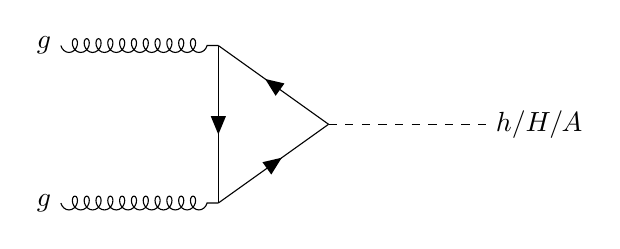
\begin{tikzpicture}[scale=2]
  \begin{feynman}
    \vertex [label=left:$g$] (a1) at (0,0);
    \vertex [label=left:$g$] (a2) at (0,1);
    \vertex (b1) at (1,0);
    \vertex (b2) at (1,1);
    \vertex (c) at (1.7,0.5);
    \vertex [label=right:$h/H/A$] (d) at (2.7,0.5);

    \diagram* {
      (a1) -- [gluon] (b1),
      (a2) -- [gluon] (b2),
      (b2) -- [fermion] (b1),
      (c) -- [fermion] (b2),
      (b1) -- [fermion] (c),
      (c) -- [scalar] (d),
    };
  \end{feynman}
\end{tikzpicture}
\caption{}
\end{subfigure}


\begin{subfigure}[b]{0.3\textwidth}
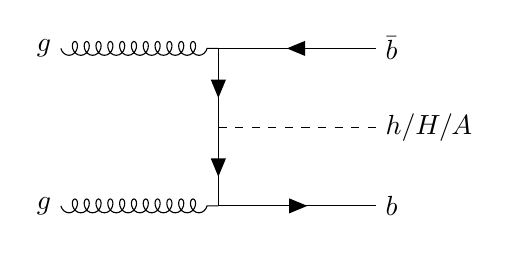
\begin{tikzpicture}[scale=2]
  \begin{feynman}
    \vertex [label=left:$g$] (a1) at (0,0);
    \vertex [label=left:$g$] (a2) at (0,1);
    \vertex (b1) at (1,0);
    \vertex (b2) at (1,0.5);
    \vertex (b3) at (1,1);
    \vertex [label=right:$b$] (c1) at (2,0);
    \vertex [label=right:$h/H/A$] (c2) at (2,0.5);
    \vertex [label=right:$\bar{b}$] (c3) at (2,1);
    \diagram* {
      (a1) -- [gluon] (b1),
      (a2) -- [gluon] (b3),
      (b3) -- [fermion] (b2),
      (b2) -- [fermion] (b1),
      (c3) -- [fermion] (b3),
      (b1) -- [fermion] (c1),
      (b2) -- [scalar] (c2),
    };
  \end{feynman}
\end{tikzpicture}
\caption{}
\end{subfigure}
\hspace{2cm}
\begin{subfigure}[b]{0.3\textwidth}
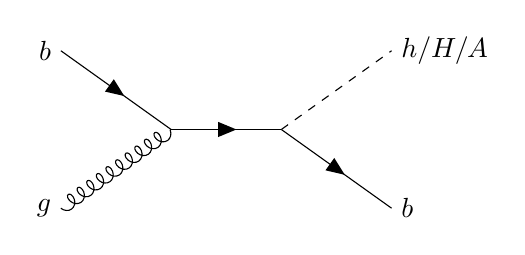
\begin{tikzpicture}[scale=2]
  \begin{feynman}
    \vertex [label=left:$g$] (a1) at (0,0);
    \vertex [label=left:$b$] (a2) at (0,1);
    \vertex (b) at (0.7,0.5);
    \vertex (c) at (1.4,0.5);
    \vertex [label=right:$b$] (d1) at (2.1,0);
    \vertex [label=right:$h/H/A$] (d2) at (2.1,1);
    \diagram* {
      (a1) -- [gluon] (b),
      (a2) -- [fermion] (b),
      (b) -- [fermion] (c),
      (c) -- [fermion] (d1),
      (c) -- [scalar] (d2),
    };
  \end{feynman}
\end{tikzpicture}
\caption{}
\end{subfigure}
\caption{Diagram (a) shows the production of neutral Higgs bosons from gluon fusion. The dominant loop contributions to this diagrams are from top-only, bottom-only and top-bottom interference. Diagrams (b) and (c) show production in association with b quarks.}
\label{fig:mssm_feynamn}
\end{figure}

With the $\tan\beta$ enhancement, the decays of additional Higgs bosons to tau leptons and bottom quarks are most likely.
Tau leptons are reconstructed more easily in the CMS detector than bottoms quarks and are much easier to separate from the large QCD multijet background produced from the high energy proton-proton collisions.

\subsection{Vector Leptoquarks}
\label{sec:vlq}

\begin{figure}[H]
\centering
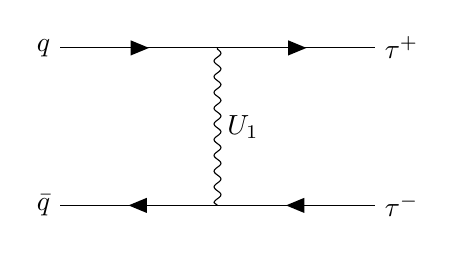
\begin{tikzpicture}[scale=2]
  \begin{feynman}
    \vertex [label=left:$\bar{q}$] (a1) at (0,0);
    \vertex [label=left:$q$] (a2) at (0,1);
    \vertex (b1) at (1,0);
    \vertex (b2) at (1,1);
    \vertex [label=right:$U_{1}$] (b3) at (1,0.5);
    \vertex [label=right:$\tau^-$] (c1) at (2,0);
    \vertex [label=right:$\tau^+$] (c2) at (2,1);

    \diagram* {
      (b1) -- [fermion] (a1),
      (a2) -- [fermion] (b2),
      (b2) -- [boson] (b1),
      (c1) -- [fermion] (b1),
      (b2) -- [fermion] (c2),
    };
  \end{feynman}
\end{tikzpicture}
\caption{Feynman diagram showing the vector leptoquark t-channel interaction that produces a tau pair from a pair of bottom quarks.}
\label{fig:leptoquark_feynman}
\end{figure}

\section{Signal Modelling}

\begin{figure}[!hbtp]
\centering
    \subfloat[]{\includegraphics[width=0.5\textwidth]{Figures/mssm_signal.pdf}}
    \subfloat[]{\includegraphics[width=0.5\textwidth]{Figures/mssm_signal.pdf}}
\caption{MSSM signal.}
\label{fig:mssm_signal}
\end{figure}

\section{Event Selection}

\begin{table}[h]
    \centering
    \begin{tabular}{|c|c|}
         \hline
         Channel & Branching Fraction  \\
         \hline
         \hline
         $\tau_h \tau_h$ & 42.0\% \\
         $e \tau_h$ & 23.1\% \\
         $\mu \tau_h$ & 22.6\% \\
         $e \mu$ & 6.2\% \\
         $e e$ & 3.2\% \\
         $\mu \mu$ & 3.0\% \\
         \hline
    \end{tabular}
    \caption{}
\end{table}

\section{Signal Extraction}

\begin{figure}[!hbtp]
\centering
    \subfloat[]{\includegraphics[width=0.5\textwidth]{Figures/vlq_signal.pdf}}
    \subfloat[]{\includegraphics[width=0.5\textwidth]{Figures/vlq_signal.pdf}}
\caption{VLQ signal.}
\label{fig:vlq_signal}
\end{figure}

\section{Background Modelling}
\subsection{Overview}
\subsection{Embedding Method}

\begin{figure}[!hbtp]
\centering
    \subfloat[]{\includegraphics[width=1.0\textwidth]{Figures/Embedding_Diagram.pdf}}
\caption{Embedding.}
\label{fig:embedding}
\end{figure}

\subsection{Fake Factor Method}
\section{Corrections}
\section{Results}
\subsection{Model Independent}

\begin{figure}[!hbtp]
\centering
    \subfloat[]{\includegraphics[width=0.45\textwidth]{Figures/postfit_lowmass_tt_nobtag_mediumpT.pdf}}
    \subfloat[]{\includegraphics[width=0.45\textwidth]{Figures/postfit_lowmass_tt_nobtag_highpT.pdf}} \\
    \subfloat[]{\includegraphics[width=0.45\textwidth]{Figures/postfit_lowmass_lt_nobtag_mediumpT.pdf}}
    \subfloat[]{\includegraphics[width=0.45\textwidth]{Figures/postfit_lowmass_lt_nobtag_highpT.pdf}} \\
    \subfloat[]{\includegraphics[width=0.45\textwidth]{Figures/postfit_lowmass_em_nobtag_mediumpT.pdf}}
    \subfloat[]{\includegraphics[width=0.45\textwidth]{Figures/postfit_lowmass_em_nobtag_highpT.pdf}}
\caption{Low mass postfit.}
\label{fig:low_mass_postfit}
\end{figure}

\begin{figure}[!hbtp]
\centering
    \subfloat[]{\includegraphics[width=0.45\textwidth]{Figures/postfit_highmass_tt_nobtag.pdf}}
    \subfloat[]{\includegraphics[width=0.45\textwidth]{Figures/postfit_highmass_tt_btag.pdf}} \\
    \subfloat[]{\includegraphics[width=0.45\textwidth]{Figures/postfit_highmass_lt_nobtag_tightmT.pdf}}
    \subfloat[]{\includegraphics[width=0.45\textwidth]{Figures/postfit_highmass_lt_btag_tightmT.pdf}} \\
    \subfloat[]{\includegraphics[width=0.45\textwidth]{Figures/postfit_highmass_em_nobtag_mediumdzeta.pdf}}
    \subfloat[]{\includegraphics[width=0.45\textwidth]{Figures/postfit_highmass_em_btag_mediumdzeta.pdf}}
\caption{High mass postfit.}
\label{fig:high_mass_postfit}
\end{figure}

\begin{figure}[!hbtp]
\centering
    \subfloat[]{\includegraphics[width=0.5\textwidth]{Figures/model_independent_limit_ggH.pdf}}
    \subfloat[]{\includegraphics[width=0.5\textwidth]{Figures/model_independent_limit_bbH.pdf}}
\caption{Model independent limits.}
\label{fig:model_independent_limits}
\end{figure}

\begin{figure}[!hbtp]
\centering
    \subfloat[]{\includegraphics[width=0.5\textwidth]{Figures/significance_plot_ggH.pdf}}
    \subfloat[]{\includegraphics[width=0.5\textwidth]{Figures/significance_plot_bbH.pdf}}
\caption{Significance.}
\label{fig:significance}
\end{figure}

\subsection{Model Dependent}

\begin{figure}[!hbtp]
\centering
    \subfloat[]{\includegraphics[width=0.5\textwidth]{Figures/vlq_bm_1.pdf}}
    \subfloat[]{\includegraphics[width=0.5\textwidth]{Figures/vlq_bm_2.pdf}}
\caption{VLQ limits.}
\label{fig:vlq_limits}
\end{figure}

\begin{figure}[!hbtp]
\centering
    \subfloat[]{\includegraphics[width=0.5\textwidth]{Figures/model-dependent_limit_mh125.pdf}}
    \subfloat[]{\includegraphics[width=0.5\textwidth]{Figures/model-dependent_limit_mh125EFT.pdf}}
\caption{MSSM limits.}
\label{fig:mssm_limits}
\end{figure}

%\newpage
%\chapter{\texorpdfstring{Search for New Physics in $\tau^+\tau^-\tau^+\tau^-$ Final States}{Search for new physics in tautautautau final states}}
\label{sec:H_A_to_4_tau_analysis}


\begin{figure}
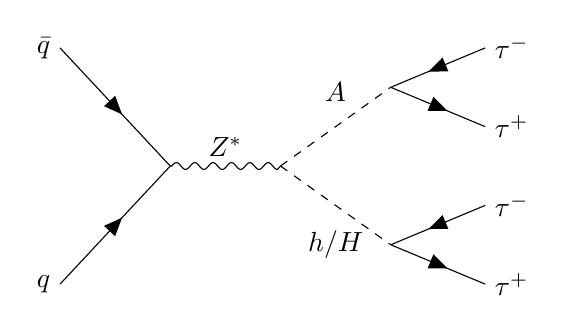
\begin{tikzpicture}[scale=2]
  \begin{feynman}
    \vertex [label=left:$q$] (a1) at (0,-0.25);
    \vertex [label=left:$\bar{q}$] (a2) at (0,1.25);
    \vertex (b) at (0.7,0.5);
    \vertex [label=above:$Z^{*}$] (b1) at (1.05,0.5);    
    \vertex (c) at (1.4,0.5);
    \vertex [label=below:$h/H$] (d11) at (1.75,0.15);
    \vertex [label=above:$A$] (d12) at (1.75,0.85);
    \vertex (d1) at (2.1,0);
    \vertex (d2) at (2.1,1);
    \vertex [label=right:$\tau^+$] (e1) at (2.7,-0.25);
    \vertex [label=right:$\tau^-$] (e2) at (2.7,0.25);
    \vertex [label=right:$\tau^+$] (e3) at (2.7,0.75);
    \vertex [label=right:$\tau^-$] (e4) at (2.7,1.25);
    \diagram* {
      (a1) -- [fermion] (b),
      (a2) -- [fermion] (b),
      (b) -- [photon] (c),
      (c) -- [scalar] (d1),
      (c) -- [scalar] (d2),
      (d1) -- [fermion] (e1),
      (e2) -- [fermion] (d1),
      (d2) -- [fermion] (e3),
      (e4) -- [fermion] (d2),
    };
  \end{feynman}
\end{tikzpicture}
\end{figure}

\begin{figure}
\begin{tikzpicture}[scale=2]
  \begin{feynman}
    \vertex (b) at (0,0.5);
    \vertex [label=above:$Z$] (b1) at (0.55,0.5);    
    \vertex (c) at (1,0.5);
    \vertex [label=right:$\tau^{-}$] (d1) at (1.7,0);
    \vertex [label=right:$\tau^{+}$] (d2) at (1.7,1);
    \diagram* {
      (b) -- [photon] (c),
      (c) -- [fermion] (d1),
      (d2) -- [fermion] (c),
    };
  \end{feynman}
\end{tikzpicture}
\end{figure}


\begin{table}[h]
    \centering
    \begin{tabular}{|c|c|}
         \hline
         Channel & Branching Fraction  \\
         \hline
         \hline
         $e \tau_h \tau_h \tau_h$ & 19.4\% \\
         $\mu \tau_h \tau_h \tau_h$ & 18.9\% \\
         $\tau_h \tau_h \tau_h \tau_h$ & 17.6\% \\
         $e \mu \tau_h \tau_h$ & 15.6\% \\
         $e e \tau_h \tau_h$ & 8.0\% \\
         $\mu \mu \tau_h \tau_h$ & 7.6\% \\
         $e e \mu \tau_h$ & 4.3\% \\
         $e \mu \mu \tau_h$ & 4.2\% \\
         $e e e \tau_h$ & 1.5\% \\
         $\mu \mu \mu \tau_h$ & 1.4\% \\
         $e e e \mu$ & 1.4\% \\
         $e e \mu \mu$ & 0.6\% \\
         $e e e \mu$ & 0.4\% \\
         $e \mu \mu \mu$ & 0.4\% \\
         $e e e e$ & 0.1\% \\
         $\mu \mu \mu \mu$ & 0.1\% \\
         \hline
    \end{tabular}
    \caption{}
\end{table}


\begin{equation}
\mathcal{L}^{\text{2HDM}}_{\text{yukawa}} = - \sum_{f=u,d,l}\Big(\frac{m_{f}}{\nu}\xi^{f}_{h}\bar{f}fh + \frac{m_{f}}{\nu}\xi^{f}_{H}\bar{f}fH -i\frac{m_{f}}{\nu}\xi^{f}_{A}\bar{f}\gamma_{5}fA\Big) - \Big[\frac{\sqrt{2}V_{ud}}{\nu}\bar{u}(m_{u}\xi^{u}_{A}P_{L} + m_{d}\xi^{d}_{A}P_{R})dH^{+} + \frac{\sqrt{2}m_{l}\xi^{d}_{A}}{\nu}\bar{\nu}_{L}l_{R}H^{+} + h.c.\Big]
\end{equation}

\begin{table}[H]
    \centering
    \begin{tabular}{p{1.5cm}|x{1.2cm}x{1.2cm}x{1.2cm}x{1.2cm}x{1.2cm}x{1.2cm}x{1.2cm}x{1.2cm}x{1.2cm}}
         \hline
          & $g_{h}^{u}$ & $g_{h}^{d}$ & $g_{h}^{l}$ & $g_{H}^{u}$ & $g_{H}^{d}$ & $g_{H}^{l}$ & $g_{A}^{u}$ & $g_{A}^{d}$ & $g_{A}^{l}$ \\
         \hline
         \hline
         Type I & $c_{\alpha}/s_{\beta}$ & $c_{\alpha}/s_{\beta}$ & $c_{\alpha}/s_{\beta}$ & $s_{\alpha}/s_{\beta}$ & $s_{\alpha}/s_{\beta}$ & $s_{\alpha}/s_{\beta}$ & $1/t_{\beta}$ & $-1/t_{\beta}$ & $-1/t_{\beta}$ \\
         Type II & $c_{\alpha}/s_{\beta}$ & $-s_{\alpha}/c_{\beta}$ & $-s_{\alpha}/c_{\beta}$ & $s_{\alpha}/s_{\beta}$ & $c_{\alpha}/c_{\beta}$ & $c_{\alpha}/c_{\beta}$ & $1/t_{\beta}$ & $t_{\beta}$ & $t_{\beta}$ \\
         Type X & $c_{\alpha}/s_{\beta}$ & $c_{\alpha}/s_{\beta}$ & $-s_{\alpha}/c_{\beta}$ & $s_{\alpha}/s_{\beta}$ & $s_{\alpha}/s_{\beta}$ & $c_{\alpha}/c_{\beta}$ & $1/t_{\beta}$ & $-1/t_{\beta}$ & $t_{\beta}$ \\
         Type Y & $c_{\alpha}/s_{\beta}$ & $-s_{\alpha}/c_{\beta}$ & $c_{\alpha}/s_{\beta}$ & $s_{\alpha}/s_{\beta}$ & $c_{\alpha}/c_{\beta}$ & $s_{\alpha}/s_{\beta}$ & $1/t_{\beta}$ & $t_{\beta}$ & $-1/t_{\beta}$ \\
         \hline
    \end{tabular}
    \caption{}
\end{table}

In the alignment limit, for the normal scenario $h_{SM}=h$, $sin(\beta-\alpha)=1$, $\implies$ $c_{\alpha}/s_{\beta}=1$, $s_{\alpha}/c_{\beta}=-1$, $s_{\alpha}/s_{\beta}=-1/t_{\beta}$, $c_{\alpha}/c_{\beta}=t_{\beta}$.

\begin{table}[H]
    \centering
    \begin{tabular}{p{1.5cm}|x{1.2cm}x{1.2cm}x{1.2cm}x{1.2cm}x{1.2cm}x{1.2cm}x{1.2cm}x{1.2cm}x{1.2cm}}
         \hline
          & $g_{h}^{u}$ & $g_{h}^{d}$ & $g_{h}^{l}$ & $g_{H}^{u}$ & $g_{H}^{d}$ & $g_{H}^{l}$ & $g_{A}^{u}$ & $g_{A}^{d}$ & $g_{A}^{l}$ \\
         \hline
         \hline
         Type I & $1$ & $1$ & $1$ & $-1/t_{\beta}$ & $-1/t_{\beta}$ & $-1/t_{\beta}$ & $1/t_{\beta}$ & $-1/t_{\beta}$ & $-1/t_{\beta}$ \\
         Type II & $1$ & $1$ & $1$ & $-1/t_{\beta}$ & $t_{\beta}$ & $t_{\beta}$ & $1/t_{\beta}$ & $t_{\beta}$ & $t_{\beta}$ \\
         Type X & $1$ & $1$ & $1$ & $-1/t_{\beta}$ & $-1/t_{\beta}$ & $t_{\beta}$ & $1/t_{\beta}$ & $-1/t_{\beta}$ & $t_{\beta}$ \\
         Type Y & $1$ & $1$ & $1$ & $-1/t_{\beta}$ & $t_{\beta}$ & $-1/t_{\beta}$ & $1/t_{\beta}$ & $t_{\beta}$ & $-1/t_{\beta}$ \\
         \hline
    \end{tabular}
    \caption{}
\end{table}

In the alignment limit, for the inverted scenario $h_{SM}=H$, $cos(\beta-\alpha)=1$ $\implies$ $c_{\alpha}/s_{\beta}=1/t_{\beta}$, $s_{\alpha}/c_{\beta}=t_{\beta}$, $s_{\alpha}/s_{\beta}=1$, $c_{\alpha}/c_{\beta}=1$.

\begin{table}[H]
    \centering
    \begin{tabular}{p{1.5cm}|x{1.2cm}x{1.2cm}x{1.2cm}x{1.2cm}x{1.2cm}x{1.2cm}x{1.2cm}x{1.2cm}x{1.2cm}}
         \hline
          & $g_{h}^{u}$ & $g_{h}^{d}$ & $g_{h}^{l}$ & $g_{H}^{u}$ & $g_{H}^{d}$ & $g_{H}^{l}$ & $g_{A}^{u}$ & $g_{A}^{d}$ & $g_{A}^{l}$ \\
         \hline
         \hline
         Type I & $1/t_{\beta}$ & $1/t_{\beta}$ & $1/t_{\beta}$ & $1$ & $1$ & $1$ & $1/t_{\beta}$ & $-1/t_{\beta}$ & $-1/t_{\beta}$ \\
         Type II & $1/t_{\beta}$ & $-t_{\beta}$ & $-t_{\beta}$ & $1$ & $1$ & $1$ & $1/t_{\beta}$ & $t_{\beta}$ & $t_{\beta}$ \\
         Type X & $1/t_{\beta}$ & $1/t_{\beta}$ & $-t_{\beta}$ & $1$ & $1$ & $1$ & $1/t_{\beta}$ & $-1/t_{\beta}$ & $t_{\beta}$ \\
         Type Y & $1/t_{\beta}$ & $-t_{\beta}$ & $1/t_{\beta}$ & $1$ & $1$ & $1$ & $1/t_{\beta}$ & $t_{\beta}$ & $-1/t_{\beta}$ \\
         \hline
    \end{tabular}
    \caption{}
\end{table}

\begin{table}[h]
    \centering
    \begin{tabular}{|c|l|}
    \hline
    Trigger & HLT Path  \\
    \hline
    SingleElectron & HLT$\_$Ele25$\_$eta2p1$\_$WPTight$\_$Gsf$\_$v\\
    \hline
    DoubleElectron & HLT$\_$Ele23$\_$Ele12$\_$CaloIdL$\_$TrackIdL$\_$IsoVL$\_$DZ$\_$v \\
    \hline
    TripleElectron & HLT$\_$Ele16$\_$Ele12$\_$Ele8$\_$CaloIdL$\_$TrackIdL \\
    \hline
    SingleMuon & HLT$\_$IsoMu24$\_$v \\
    & OR \\
    & HLT$\_$IsoTkMu24$\_$v \\
    \hline
    DoubleMuon & HLT$\_$Mu17$\_$TrkIsoVVL$\_$Mu8$\_$TrkIsoVVL($\_$DZ)$\_$v \\
    & OR \\
    & HLT$\_$Mu17$\_$TrkIsoVVL$\_$TkMu8$\_$TrkIsoVVL($\_$DZ)$\_$v \\
    \hline
    TripleMuon & HLT$\_$TripleMu$\_$12$\_$10$\_$5 \\
    \hline
    SingleTau & HLT$\_$VLooseIsoPFTau120$\_$Trk50$\_$eta2p1$\_$v \\
    & OR \\
    & HLT$\_$VLooseIsoPFTau140$\_$Trk50$\_$eta2p1$\_$v \\
    \hline
    DoubleTau & HLT$\_$DoubleMediumIsoPFTau35$\_$Trk1$\_$eta2p1$\_$Reg$\_$v \\
    \hline
    Electron Tau Cross & HLT$\_$Ele24$\_$eta2p1$\_$WPLoose$\_$Gsf$\_$LooseIsoPFTau20$\_$SingleL1$\_$v \\
    \hline
    Muon Tau Cross & HLT$\_$IsoMu19$\_$eta2p1$\_$LooseIsoPFTau20$\_$SingleL1$\_$v \\
    \hline
    \end{tabular}
    \caption{2016 HLT paths.}
\end{table}

\begin{table}[]
\begin{tabular}{|c|c|c|}
\hline
$e$ & $\mu$ &  $\tau_{h}$ \\
\hline
\hline
$p_{T} > 15$ GeV & $p_{T} > 15$ GeV & $p_{T} > 20$ GeV \\
$|\eta| < 2.5$ & $|\eta| < 2.4$ & $|\eta| < 2.3$ \\
MVA 90\% WP & Medium ID & HPS algorithm \\
$d_{xy} < 0.045$ cm & $d_{xy} < 0.045$ cm & deepTauVSjet Loose WP \\
$d_{z} < 0.2$ cm & $d_{z} < 0.2$ cm & deepTauVSele VVLoose WP \\
$I_{rel} < 0.15$ & $I_{rel} < 0.15$ & deepTauVSmu VLoose WP \\
\hline
\end{tabular}
\end{table}

\section{Introduction}
\section{Signal Modelling}
\section{Event Selection}
\section{Signal Extraction}
\section{Background Modelling}
\subsection{Overview}
\subsection{Machine Learning Fake Factor Method}
\section{Corrections}
\section{Results}

%\newpage
%\chapter{Conclusion}

\section{Global Interpretations of Results}

\begin{figure}[!hbtp]
\centering
    \subfloat[]{\includegraphics[width=0.7\textwidth]{Figures/md_mphi100_hb.pdf}} \\
    \subfloat[]{\includegraphics[width=0.7\textwidth]{Figures/md_mphi200_hb.pdf}} 
\caption{}
\label{fig:4tau_md_hb}
\end{figure}

\section{Outlook}
\newpage
\bibliographystyle{ieeetr}
\bibliography{bibs/sample}

\end{document}